%%% Local Variables: 
%%% mode: latex
%%% TeX-master: "../KanjiHWR"
%%% End: 

\chapter{Technical Design of the Application}
\label{chap:technicaldesign}

The focus of this chapter is on the general architectural choices made during
the development of the system. In this chapter, the technical design aspects 
of the application are described. The general system architecture is layed out in
section~\ref{sec:systemarchitecture}. It contains the global view on the software
architecture in section~\ref{sec:globalarchitecture}, the data flow in within
the system in section~\ref{sec:arch:systemdataflow} and describes the design
of the individual modules in section~\ref{sec:arch:softwaremodules}.
Section~\ref{sec:frameworkanddevices} describes the technical set-up and 
framework choices. However, the handwriting recognition engine is described 
in detail in a separate 
section~(see chapter~\ref{chap:handwritingrecognitionengine}).

\section{System Architecture}
\label{sec:systemarchitecture}

The system architecture of the Kanji Coach follows the requirements of an 
e-learning environment dealing with the specific difficulties for learners 
of the Japanese script (see chapter~\ref{chap:japanasescript}) and those of an 
on-line handwriting recognition. Techniques of handwriting recognition are 
reviewed in chapter~\ref{chap:onlinehwr}. The general requirements of an 
e-learning application are presented in chapter~\ref{chap:elearning}. 
The resulting specific conceptual design choices have been 
layed out in chapter~\ref{chap:conceptualdesignofkanjicoach}.

\subsection{Global Architecture}
\label{sec:globalarchitecture}

The global architecture of the application follows the Model-View-Controller
(MVC) design pattern. This paradigm is used as a general model, however, 
it is not implemented the strict way proposed by~\shortcite{Krasner1988}.
Figure~(\ref{fig:modelviewcontroller}) shows the general set-up of the 
MVC design pattern after~\shortcite{Krasner1988}. xxx: Also 
figure~(\ref{fig:modelviewcontroller2}) - decide how it should be done and use
the appropriate gfx. xxx!

%xxx Make this a graphic, not a photographic image of a graphic 
\begin{figure}[htbp]
\begin{center}
\includegraphics[scale=0.5]{images/TechnicalDesign/MVC.png}
\caption{The Model-View-Controller paradigm}
\label{fig:modelviewcontroller}
\end{center}
\end{figure}

%xxx Make this a graphic, not a photographic image of a graphic 
\begin{figure}[htbp]
\begin{center}
\includegraphics[scale=0.5]{images/TechnicalDesign/ModelViewControllerDiagram.png}
\caption{The Model-View-Controller paradigm AGAIN!}
\label{fig:modelviewcontroller2}
\end{center}
\end{figure}

A global overview of the system architecture can be seen in 
figure~(\ref{fig:globalarchitecture}).
%xxx Make this a graphic, not a photographic image of a graphic 
\begin{figure}[htbp]
\begin{center}
\includegraphics[scale=0.5]{images/TechnicalDesign/GlobalArchitecture.png}
\caption{The global architecture of the software system}
\label{fig:globalarchitecture}
\end{center}
\end{figure}

\subsection{System Data Flow}
\label{sec:arch:systemdataflow}
The system data flow is shown in figure~(\ref{fig:systemdataflow}).
%xxx Make this a graphic, not a photographic image of a graphic 
\begin{figure}[htbp]
\begin{center}
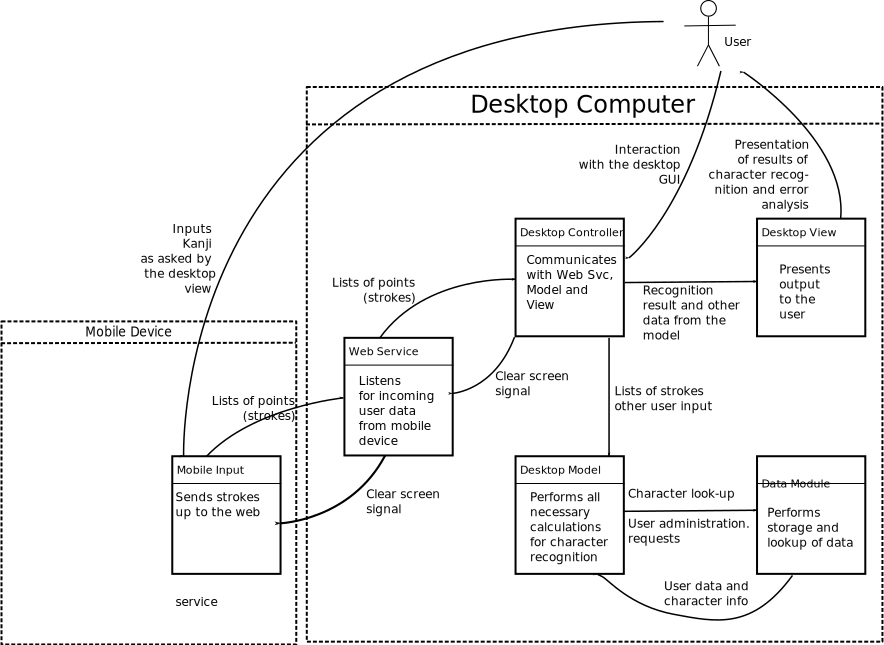
\includegraphics[scale=0.5]{images/TechnicalDesign/SystemDataFlow.png}
\caption{The data flow within the software system}
\label{fig:systemdataflow}
\end{center}
\end{figure}

\subsubsection{Communication}
\label{sec:communication}

\subsubsection{Recognition Data Flow}
\label{sec:arch:recognitiondataflow}

\subsubsection{Learning Data Flow}
\label{sec:arch:learningdataflow}

\subsection{Software Modules}
\label{sec:arch:softwaremodules}

\subsubsection{Mobile GUI}
\label{sec:arch:mobilegui}

\subsubsection{Desktop GUI}
\label{sec:arch:desktopgui}

\subsubsection{Web Service}
\label{sec:arch:webservice}

\subsubsection{Recognition Module}
\label{sec:arch:recognitionmodule}

\subsubsection{Learning Module}
\label{sec:arch:learningmodule}

\section{Framework and Devices}
\label{sec:frameworkanddevices}

\subsection{Operating System}
\label{sec:operatingsystem}

\subsection{Framework}
\label{sec:framework}

.NET vs. Java etc.

\subsection{Desktop Computer}
\label{sec:desktopcomputer}

\subsection{Pen Input Device}
\label{sec:peninputdevice}

\subsubsection{Stylus Input}
\label{sec:stylusinput}






